%&pdflatex
%% filename: amsart-template.tex, version: 2.1
\documentclass{amsart}
\usepackage{hyperref}
\usepackage{inputenc}
\usepackage{graphicx}
\usepackage{bbm}

\newtheorem{theorem}{Theorem}[section]
\newtheorem{lemma}[theorem]{Lemma}
\theoremstyle{definition}
\newtheorem{definition}[theorem]{Definition}
\newtheorem{example}[theorem]{Example}
\newtheorem{xca}[theorem]{Exercise}
\theoremstyle{remark}
\newtheorem{remark}[theorem]{Remark}
\numberwithin{equation}{section}
\setlength{\parindent}{0pt} % turn off auto-indent

\graphicspath{ {./} }

\begin{document}

\title{Assignment 1: Theory of Multi Layer Perceptrons [IFT6135]}

\author{Joseph D. Viviano}
\address{Universit\'e de Montr\'eal}
\curraddr{}
\email{joseph@viviano.ca}
\thanks{}
\date{Feburary 2018}

\maketitle

\section{Neural Network Classification}

%https://deepnotes.io/softmax-crossentropy
%
(a) $\sigma(z) = 1/(1 + e^{-z})$ is an appropriate activation function for binary
classification (i.e., the sigmoid activation function). \\

(b) $\sigma(z)$ (above) outputs numbers on the interval $[0, 1]$ and can be
interpreted as a probability. \\

(c) $L= -y\log g(z) - (1-y)\log(1-g(z))$ is the cross entropy loss. \\

(d) For cross entropy loss, $df/da=g(a)(1-g(a))$, and $\partial L/\partial a = f-y$ \\

(e) $L=1/2(y-f)^2$ is the mean squared error loss (assuming a single example). \\

(f) For mean squared error loss, $\partial L/\partial a = -(y-f)g(a)(1-g(a))$ \\

(g) For binary classification, we want our responses to be bounded between two
values, the extremes representing each class and the distance to each
representing our certianty of choosing one class versus the other class. The
cross entropy loss outputs a probability, which fulfills the aformentioned
requirements, while the mean squared error loss is unbounded, making it a less
suitable loss for binary classification. One could define a threshold on which
to binarize the outputs to produce a classification, but if we were to use
a sigmoid output unit (or another option with similar properties), the units
would saturate quickly and very small gradients (and therefore little learning)
would be produced if the neuron's mean squared error loss ever grew too large. \\


\section{Neural Network Representation}

\textit{Fill the parameters of a MLP binary classifier using a Heavyside step
function, two input neurons, three hidden neurons, and one output neuron.} \\

Three decision boundaries are required to seperate all samples by their class.
First we define four relevant points: \\

%  (x , y)
$p_1 = (-4, 0)$ \\
$p_2 = (0, -4)$ \\
$p_3 = (4, 0)$ \\
$p_4 = (0, 4)$ \\

And second, we define the three decision boundaries: \\

$d_1 = \overrightarrow{p1p2}$ \\ % yint = -4
$d_2 = \overrightarrow{p2p3}$ \\ % yint = -4
$d_3 = \overrightarrow{p3p4}$ \\ % yint =  4

These decision boundaries are computed by the hidden layer of our network. Each
neuron $i$ recieves two inputs: $x_{1i}$ and $x_{2i}$ modulated by weights
$w_{1i}$ and $w_{2i}$. $d_1$ has slope = -1 and passes through y=-4,
$d_2$ has slope = 1 and passes through y = -4, and $d_3$ has
slope = -1 and passes through y = 4. Therefore the three decision planes can be
expressed using the form $y = mx + b$ as so: \\

$d_1 = -1x - 4$ \\
$d_2 = 1x - 4$ \\
$d_3 = -1x + 4$ \\

Since the weights define the slope of each decision boundary, they are trivial
to derive: \\

$w_{11} = -1$ and $w_{21} = 1$ for $d_1$, \\
$w_{12} = 1$ and $w_{22} = 1$ for $d_2$, \\
$w_{13} = -1$ and $w_{23} = 1$ for $d_3$. \\

The bias of each decision boundary defines it's offset from the origin, or the
euclidean distance between the origin and the closet point of the decision
boundary. Therefore, the biases for these decision boundaries ${b_1, b_2, b_3}$
are set to be $-2$, $-2$, and $2$, respectively.\\

Finally, these decision boundaries must be added and subtracted from one another
using the output layer weights ${u_1, u_2, u_3}$, and the bias of the output
neuron $c$ set's the default state of the decision space. Therefore, to carve
out the required boundary, we set the output biases to ${u_1 = -1}$ to remove
the lower boundary, ${u_2 = -1}$ to remove the side boundary, and ${u_3 = 1}$ to
 add the top boundary, which leaves us with the correct decision boundary. The
output bias ${u}$ must be set $-1 < u < 0$ so that these subtractions and
additions produce the correct behaviour after the Heavyside step function, which
sets all values less that 0 to 0, and all values greater than 0 to 1. \\

Please see \textbf{figure 1} for an illustration incorperating these parameters.
\begin{figure}[h]
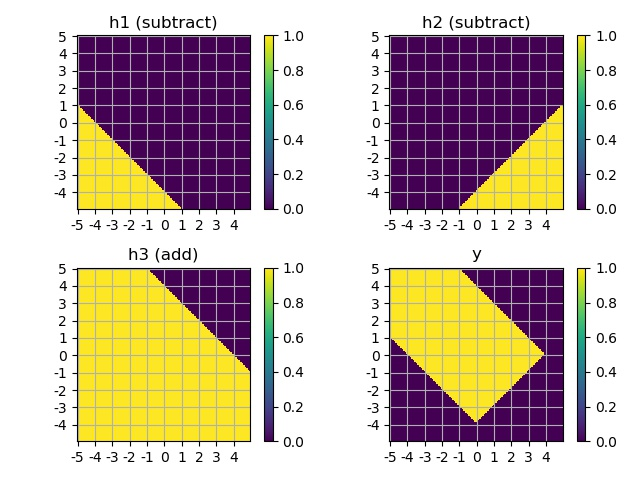
\includegraphics[width=100mm]{heavyside_decision_boundary}
\caption{Heavyside decision boundary.}
\label{Figure 1}
\end{figure}


\section{Activation Functions}

(a) \textit{Show that $ReLU'(x)$ is given by the Heavyside step function $H(x)$}.\\

The heavyside step function is always 0 when $x < 0$, always 1 when $x > 0$,
and vertical (undefined) at $x = 0$. $ReLU(x) = max(0, x)$ is 0 when $x < 0$,
some linear function $y = f(x)$ when $x > 0$, and 0 when $x = 0$. Therefore the
derivative of the ReLU function is defined everywhere except at $x = 0$, since
that one location is not continuous. Furthermore when $x < 0$ $dy/dx = 0$ since
it is constant, and when $x > 0$, $dy/dx = 1$ since it is the derivative of a
single variable. Assembling these pieces, we get the heavyside step function. \\

(b) Two definitions of ReLU using the Heavyside step function include
$xH(x)$ and $x^{H(x)}-\mathbbm{1}_{x\leq0} $. \\

(c) \textit{Show the sigmoid function behaves asymptotically like H(x)}. \\

As $\lim_{a\rightarrow\infty} 1/(1+e^{-x})$, $\sigma(x)$ approaches 1 because
the term $e^{-x}$ quickly approaches 0, and conversly, as
\lim_{a\rightarrow-\infty} 1/(1+e^{-x}),  $\sigma(x)$ approaches 0 because the
denominator grows very large. Therefore $\sigma(x)$ behaves asymtotically as the
$H(x)$ function. \\

(d) \textit{Show H'(x) is given by the dirac delta function}. \\

First, observe that the Heavyside function is constant everywhere, excecpt at
$x = 0$. Therefore $H'(x<0) = 0$ and $H'(x>0) = 0$. Second, at $x = 0$, the
slope of the Heavyside function is $\infty$ (a vertical line), so $H'(x=0) =
\infty$. If we combine these three intervals, $x<0$, $x=0$, and $x>0$, we get
the dirac function, which is equal to $H'(x)$:

\begin{equation}
H'(x) = \delta(x) = \begin{cases} +\infty, & x = 0 \\ 0, & x \ne 0 \end{cases}.
\end{equation} \\

If we integrate over any area where the entire density of the distribution is
concentrated at x=0, we end up with the second property of the Dirac function
since the sum of the area under an integral is always equal to 1:

\begin{equation}
\int_{-\infty}^\infty H'(x) \, dx = \int_{-\infty}^\infty \delta(x) \, dx = 1.
\end{equation} \\


\section{Gradients and Networks}

(a) For the softmax function $\sigma(\mathbf{z})_j = \frac{e^{z_j}}{\sum_{k=1}^K e^{z_k}}$,
the jacobian is $J = (\partial softmax/\partial z)_{ij}$.

\begin{equation}
\frac{\partial softmax_i(z)}{\partial z_j} = \frac{\delta_{ij}e^{z_i}\sum_k e^{z_k} - e^{z_i}e^{z_j}}{\left(\sum_k e^{z_k}\right)^2} \\
\end{equation}

Which simplifies to:

\begin{equation}
\frac{\partial softmax_i(z)}{\partial z_j} = softmax_i(z) (\delta_{ij}-softmax_j(z)).
\end{equation}

In both cases $\delta_{ij}$ is the Kronecker delta, which evaluates to $1$ if
$i=j$ and is $0$ otherwise. \\

(b)

Observe the jacobian as a matrix equation. For berivity we represent $softmax$ as $s$ below: \\

\begin{bmatrix}
{s_{1}(1-s_{1}(z)) & -s_1s_2           & \cdots & -s_1s_n \\
{-s_2s_1           & s_{2}(1-s_{2}(z)) & \cdots & -s_2s_n \\
{\vdots            & \vdots            & \ddots & \vdots  \\
{s_{n}(1-s_{1}(z)) & -s_ns_2           & \cdots & s_{n}(1-s_{n}(z)) \\
\end{bmatrix} \\
\\

(c) The jacobian of the logistic sigmoid applied element-wise to a vector $x$ is
the diagonal of the above matrix, i.e., $diag(softmax_i(z) (\delta_{ij}-softmax_j(z)))$. \\

(d) To see that $J_y(x) g_y = g_y \circ \sigma'(x)$, first expand
$g_y$ to the matrix $J_y (g_y_1,...,g_y_n)^T$, and multiply $\sigma'(x)$ into
each element: $(\sigma'(x_1)g_y_1,...,\sigma'(x_n)g_y_n)^T$. \\
From this, we see $(g_y_1,...,g_y_n)^T \odot(\sigma'(x_1),...,\sigma'(x_n))^T$. \\

If $J_y(x)$ were the jacobian of the softmax function, this does not hold
because $J_y$ would not be a diagonal matrix. \\


\section{Softmax Activation Function}

(a) The softmax is invariant under translation, i.e., when a constant $c$ is
added to all values of $x$, i.e, $softmax(x+c) = e^{x_i+c}/\sum_k e^{x_k + c}$,
because it is normalized by the sum of all $e^x_i$, i.e., if all values are
equally shifted by some constant $c$, they will simple be range-normalized back to the
range $[0, 1]$. \\

(b) The softmax function is not invariant under multiplication, because when
$-1 < x < 1$, multiplication will shrink $|x|$, whereas when $x > 1 \vee X < -1$,
multiplcation will increase $|x|$. Multiplication would have the effect of making
the softmax more certian of the most likely output, i.e., it would sharpen
the distribution of probabilities computed by the softmax. \\

(c) The sigmoid function is equivilant to a 2-class softmax. Let me show you: \\

First, observe the sigmoid: $\sigma(z) = 1/(1 + e^{-z})$. Isn't it nice? Second, observe the
general form of the k-class softmax: $\frac{e^{x_i}}{\sum_{i=1}^k e^{x_i}}$. \\

Now let's split up the softmax into the two-class case:\\

\begin{equation}
softmax(x) = \left(\frac{e^{x_1}}{e^{x_1} + e^{x_2}} + \frac{e^{x_2}}{e^{x_1} + e^{x_2}}\right)
\end{equation}

So for the $x_1$ case: \\

\begin{equation}
softmax(x_1) =       \frac{e^{x_1}}{e^{x_1} + e^{x_2}}
             =       \frac{1}{1 + e^{x_2-x_1}}
             =       \frac{1}{1 + e^{-x_1-x_2}}
             =       \frac{1}{1 + e^{-z}}
\end{equation}

Therefore if $z = x_1 - x_2$, $\sigma(z) = softmax(x_1)$. We can compute a
similar equality for $softmax(x_2)$: \\

\begin{equation}
softmax(x_2) =       \frac{e^{x_2}}{e^{x_1} + e^{x_2}}
             =       \frac{1}{e^{x_1-x_2} + 1}
             =   1 - \frac{1}{1 + e^{-x_1-x_2}}
             =   1 - \frac{1}{1 + e^{-z}}

\end{equation}

Therefore $1- \sigma(z) = softmax(x_2)$, and more completely: \\

\begin{equation}
\left( \sigma(z), 1-\sigma(z)\right) = \left( softmax(x_1), softmax(x_2) \right)
\end{equation}\\

(d) Note that in the previous 2-class example, we divide each element of the softmax
vector by it's numerator, which results in the term $1 + e^{-x_1-x_2}$ in the
demoninator. It is not hard to see that, for the three class case, if we were
to divide the fraction by the same numerator, we would be left with
$1 + e^{-x_1-x_2} + e^{-x_1-x_3}$ in the demoninator. We could therefore assign
two variables $a=-x_1-x_2, b=-x_1-x_3$, to represent the 3 class
softmax as 2 variables $a$ and $b$. By induction, we can see that the $k$-class
softmax can be represented as using variables $\left{a, b, ..., k-1\right}$.  \\


\section{Using Cross Entropy (Negative Log Likelihood) for Real-Valued Data}

%https://stats.stackexchange.com/questions/265966/why-do-we-use-kullback-leibler-divergence-rather-than-cross-entropy-in-the-t-sne
%https://tdhopper.com/blog/cross-entropy-and-kl-divergence/
(a) \textit{Derive the cross-entropy cost function using the maximum likelihood
principle for x}\\

We set $prob(x=1) = p$, and $prob(x=0) = 1-p$ \\

This can be expressed as the bernoulli distribution $f(x;p):
$p^x(1-p)^{1-x}$ for x \in {0,1}$. \\

This allows us to express this as the negative log likelyhood seen in
question 1: $-x\log p + (1-x)\log(1-p)$, aka the cross entropy loss. \\

(b) Here I present a probabilistic interpretation of cross-entropy
using the KL divergence between two distributions. According to
\href{https://en.wikipedia.org/wiki/Cross_entropy}{wikipedia}, the relationship
between Cross-entropy and K-L divergence is: \\

\begin{equation}
H(p, q) = \operatorname{E}_p[-\log q] = H(p) + D_{\mathrm{KL}}(p \| q)=-\sum_x p(x)\log q(x)
\end{equation}

Where $p$ and $q$ are two probability distributions (meaning
$p \in [0,1], q \in [0,1]$). $p$ represents the likelyhood
of $x$ truly being 1, and $q$ represents the probability of predicting that $x$ is 1.
$H(p)$ is the entropy of p, and $H(p, q)$ is the cross-entropy of these two
probability distributions. Therefore, the cross entropy is simply the sum of the
$H(p)$, and the K-L divergence ${p \| q}$, a measure of the difference between
the distributionn of model predictions $q$ and the true distribution $p$. \\

The K-L divergence for these two distributions is:

\begin{equation}
D_{\mathrm{KL}}(p\|q) = - \sum_x p(x) \, \log\frac{q(x)}{p(x)}
\end{equation}

and the entropy for $p$ is:

\begin{equation}
H(p) = \sum{p(x) \log p(x)}
\end{equation}

therefore it is trivial to show:

\begin{equation}
\sum_x{p(x) \log p(x)} - \sum_x p(x) \, \log\frac{q(x)}{p(x)} = -\sum_x p(x)\log q(x)
\end{equation}


\section{Q7: Deriving the Glorot Initialization Scheme}

%http://andyljones.tumblr.com/post/110998971763/an-explanation-of-xavier-initialization
%
%NB different assumptions for each section \\
%\begin{equation}
%\operatorname{Var}(X) &= \operatorname{E}\left[(X - \operatorname{E}[X])^2\right] \\
%&= \operatorname{E}\left[X^2 - 2X\operatorname{E}[X] + \operatorname{E}[X]^2\right] \\
%&= \operatorname{E}\left[X^2\right] - 2\operatorname{E}[X]\operatorname{E}[X] + \operatorname{E}[X]^2 \\
%&= \operatorname{E}\left[X^2 \right] - \operatorname{E}[X]^2
%\end{equation}

The Glorot initialization scheme was developed to work on the sigmoid
activation function, assuming all weights were in the linear regime of the
sigmoid. The goal of this initialization scheme is to ensure that all layers
have a $\operatorname{E} = 0$ and $\operatorname{Var}(X) = 1$. \\

The values in layer $Y$ will be the result of all $n$ layers before it: \\

\begin{equation}
Y_i = W_1X_1 + W_2X_2 + \dotsb + W_n X_n
\end{equation}

Where $X_i$ is the inputs to that layer and $W_i$ are the weights into that layer.
The variance of $W_iX_i$: \\

\begin{equation}
\text{Var}(W_iX_i) = E[X_i]^2 \text{Var}(W_i) + E[W_i]^2 \text{Var}(X_i) + \text{Var}(W_i)\text{Var}(i_i)
\end{equation}

Since we want the mean to be zero, we can remove all terms with $\operatorname{E}$:

\begin{equation}
\text{Var}(W_iX_i) = \text{Var}(W_i)\text{Var}(X_i)
\end{equation}

Next we assume that these are uncorrelated variables, so the variance of $Y$ is
simply the sum of all $n$ input varainces:\\

\begin{equation}
\text{Var}(Y_i) = \sum_n{\text{Var}(W_i)\text{Var}(X_i)}
\end{equation}

If we want $\text{Var}(Y_i)$ to be equal to $\text{Var}(X_i)$, we therefore need
$\text{Var}(W_i)$ to be equal to $\frac{1}{n}$, so the terms cancel out. \\

This is true for both the forward pass and backward pass of backpropogation
independently, with each serving as an input to layer $Y$, we simply take the
sum of the inverse of of the weight counts for the forward and backward pass
($n_{i}$ and $n_{i+1}$):

\begin{equation}
\text{Var}(W_i) = \frac{2}{n_{i} + n_{i+1}}
\end{equation}

In the case of ReLU, the linear assumption used in the original paper does not
hold (recall the paper only analyzed the linear regime of the sigmoid activation
function around zero). With ReLU, all values below $x = 0$ are 0, while all
values above are $x$, which effectively cuts our variance in half since our
initialized values are centered around zero. Therefore we must double our weight
variance to keep the variance constant throughout the layers:

\begin{equation}
\text{Var}(W_i) = \frac{4}{n_{i} + n_{i+1}}
\end{equation}

\end{document}

% End of amsart-template.tex
